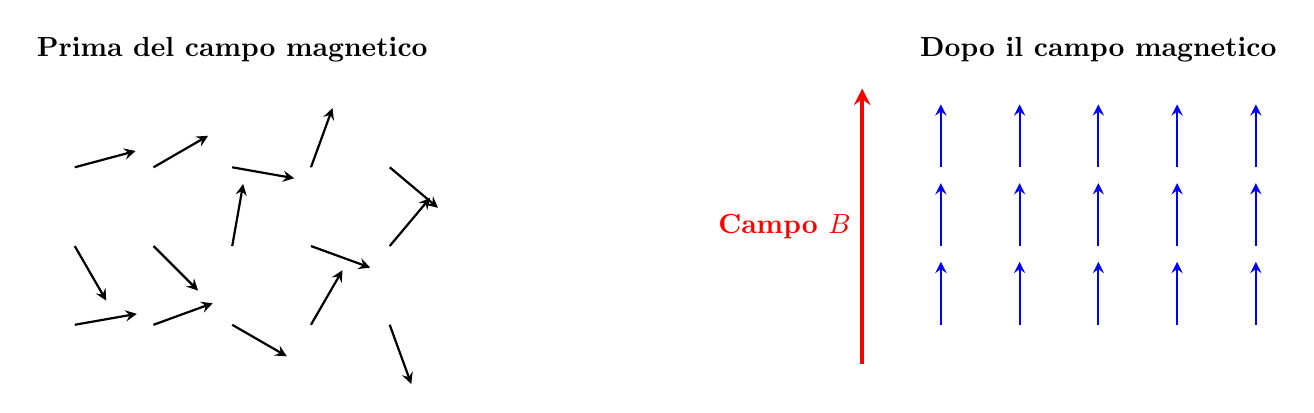
\begin{tikzpicture}[>=stealth, scale=1]

% Titoli
\node at (-8,3.5) {\textbf{Prima del campo magnetico}};
\node at (3,3.5) {\textbf{Dopo il campo magnetico}};

% Prima del campo magnetico (spin disordinati su griglia, molto a sinistra)
\foreach \x/\y/\angle in {-9/0/20, -8/0/-30, -7/0/60, -6/0/-70, -10/0/10,
                          -9/1/-45, -8/1/80, -7/1/-20, -6/1/50, -10/1/-60,
                          -9/2/30, -8/2/-10, -7/2/70, -6/2/-40, -10/2/15}
    \draw[->, thick] (\x,\y) -- ++({0.8*cos(\angle)},{0.8*sin(\angle)});

% Dopo il campo magnetico (spin allineati verso l'alto)
\foreach \x in {1,2,3,4,5}
  \foreach \y in {0,1,2}
    \draw[->, thick, blue] (\x,\y) -- ++(0,0.8);

% Campo magnetico indicato
\draw[->, ultra thick, red] (0,-0.5) -- (0,3) node[midway,left] {\textbf{Campo $B$}};

\end{tikzpicture}